
\section{The Standard Model}
The standard model\cite{SMref1}\cite{SMref2}\cite{SMref3}, forming up since 1970s, is now the fundamental of elementary particle physics. After half a century's development based on the quantum field theory, nowadays the standard model is a framework that is confirmed by the observatory of numerous experiments and can be used to explain most of the particle behaviors and interactions in this universe. In the standard model there are generally 2 categories of particles: fermions and bosons. Fermions, which always have half-integer spins, make up all the matter in the universe. On the other hand, bosons with integer spins mediate the interactions among the fermions, and the interactions here includes electro-magnetic interaction, weak interaction and strong interaction. Figure~\ref{fig:smpfamily} shows all the particles that have been discovered and included in the standard model.
\begin{figure}[htbp]
\begin{center}
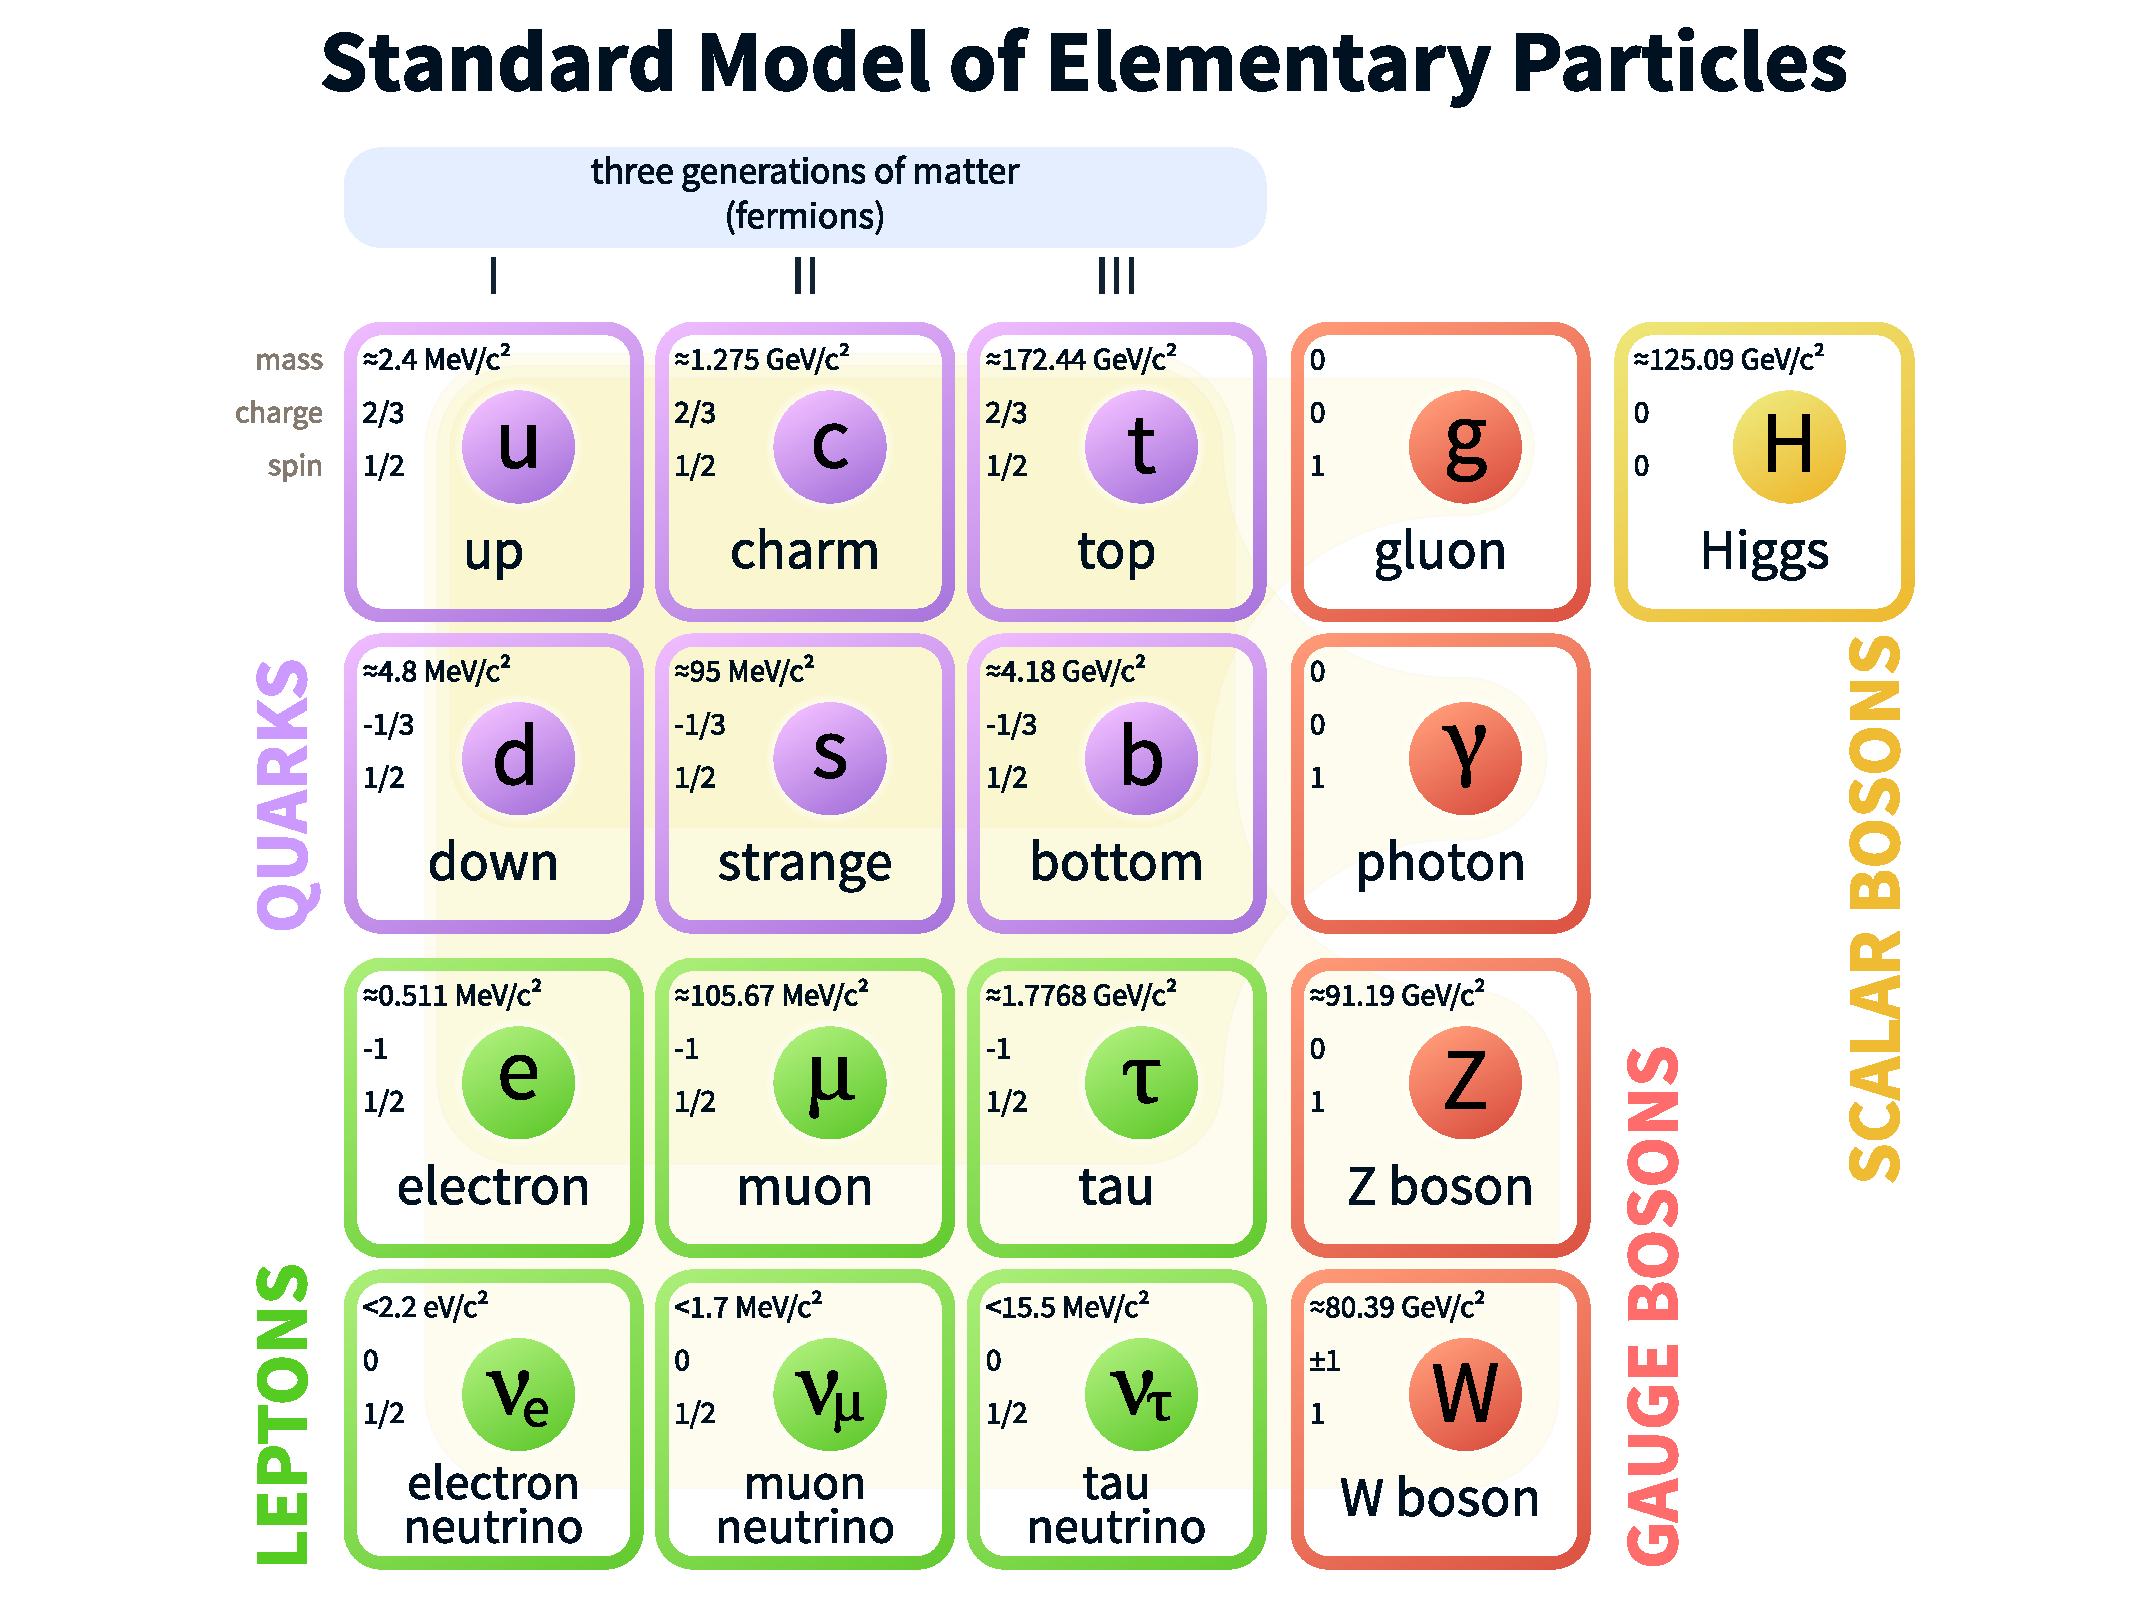
\includegraphics[width=0.72\linewidth]{figures/smpfamily.pdf}
\caption{The standard model contains 3 generations' leptons and quarks, 4 kinds of vector bosons and the higgs boson.}
\label{fig:smpfamily}
\end{center}
\end{figure}

\subsection{Fermions}
Fermions are the particles that follow Fermi–Dirac statistics and obey the Pauli exclusion principle. Every fermion has its anti particle, which is a fermion with opposite charge. The elementary fermions in the standard model includes leptons and quarks, both of them consist of 3 generations and each generation consists of 2 flavors of fermions. Every elementary fermion in the standard model has half spin. 
\subsubsection{Lepton}
The leptons are the fermions that never participate in strong interaction. 
\subsubsection{Quark}
A quark can participate in any of the 3 interactions in standard model. 
\subsection{Bosons and the interactions}
\subsubsection{Vector Bosons}
\subsubsection{The Higgs}

\section{The Limit of Standard Model}


\section{Bulk RS Graviton Model and extra dimension}



